\documentclass{beamer}

%%%%%%%%%%%%%%%%%%%%%%%%%%%%%%%%%%%%%%%%%%%%%%%%%%%%%%%%%%%%%%%%%%%%%%%
% Definicion de paquetes
\usepackage{minted}
\usepackage[utf8]{inputenc}
\usepackage[spanish]{babel}
\usepackage{hyperref}
\usepackage[nodayofweek,level]{datetime}
\usepackage{xargs}
\usepackage[colorinlistoftodos,prependcaption,textsize=tiny]{todonotes}
\presetkeys{todonotes}{inline}{}
\usepackage{pgfpages}
\usepackage[pdf]{graphviz}
%%%%%%%%%%%%%%%%%%%%%%%%%%%%%%%%%%%%%%%%%%%%%%%%%%%%%%%%%%%%%%%%%%%%%%%
% Definición de comandos
\setlength{\marginparwidth}{2cm}
% \unsure{I'm not sure}
\newcommandx{\unsure}[2][1=]{\todo[linecolor=red,backgroundcolor=red!25,bordercolor=red,#1]{#2}}
% \change{This must be changed}
\newcommandx{\change}[2][1=]{\todo[linecolor=blue,backgroundcolor=blue!25,bordercolor=blue,#1]{#2}}
% \info{Just information}
\newcommandx{\info}[2][1=]{\todo[linecolor=green,backgroundcolor=green!25,bordercolor=green,#1]{#2}}
% \improvement{THIS must be improved}
\newcommandx{\improvement}[2][1=]{\todo[linecolor=orange,backgroundcolor=orange!25,bordercolor=orange,#1]{#2}}
\newcommandx{\thiswillnotshow}[2][1=]{\todo[disable,#1]{#2}}
\newcommand{\mydate}{\formatdate{15}{12}{2021}}

\graphicspath{ {images/} }

%%%%%%%%%%%%%%%%%%%%%%%%%%%%%%%%%%%%%%%%%%%%%%%%%%%%%%%%%%%%%%%%%%%%%%%
% Beamer
\usetheme{Madrid}
\AtBeginEnvironment{minted}{\fontsize{12}{12}\selectfont}
% \setbeameroption{show notes on second screen=right}
% \setbeameroption{show only notes}
% \setbeameroption{show notes}
% \setbeamertemplate{note page}[default]
\setbeamertemplate{caption}{\raggedright\insertcaption\par}
%%%%%%%%%%%%%%%%%%%%%%%%%%%%%%%%%%%%%%%%%%%%%%%%%%%%%%%%%%%%%%%%%%%%%%%
% Título
\title[CAP]{Paso de mensajes con Erlang}
\author[M. Ruiz (UCM)]{Miguel Emilio Ruiz Nieto}
\date{\mydate}
%%%%%%%%%%%%%%%%%%%%%%%%%%%%%%%%%%%%%%%%%%%%%%%%%%%%%%%%%%%%%%%%%%%%%%%
%% Empieza el documento
\begin{document}
  \begin{frame}
    \titlepage
  \end{frame}

  \begin{frame}{Contenidos}
    \tableofcontents[hideallsubsections]
  \end{frame}

  \section{Introducción}
  \begin{frame}{Introducción}
    \begin{itemize}
      \item Hemos visto cómo funciona en computación distribuida el paso de
      mensajes qué problemas puede resolver
      \item Ahora nos centraremos en cómo funciona el paso de mensajes en Erlang
      y sus aplicaciones
    \end{itemize}
  \end{frame}

  \section{Erlang}
    \subsection{Historia}
      \begin{frame}{Erlang}
        \begin{itemize}
          \item Lenguaje de programación desarrollado en Ericsson
          \item Orientado a sistemas distribuidos:
          \begin{itemize}
            \item Modelo de actores
            \item Paso de mensajes
            \item Tolerancia a fallos
            \item Alta disponibilidad
            \item Filosofía ``Let it crash''
          \end{itemize}
        \end{itemize}
      \end{frame}

      \subsection{Actores}
      \begin{frame}{Erlang. Modelo de actores}
        \begin{figure}
          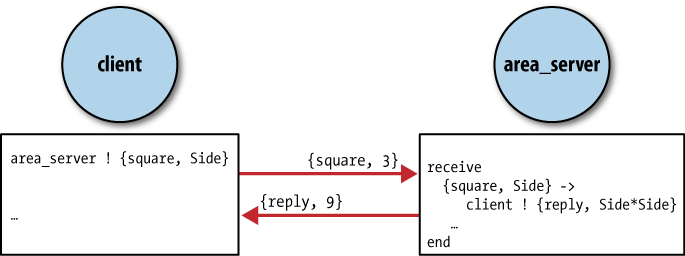
\includegraphics{actor-modelling.png}
        \end{figure}
      \end{frame}

      \begin{frame}{Erlang. Paso de mensajes}
        \begin{figure}
          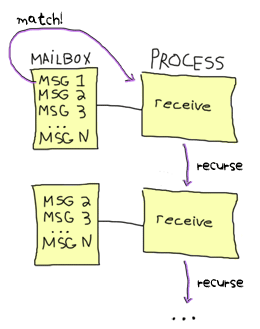
\includegraphics[width=0.45\textwidth]{msg-match.png}
        \end{figure}
      \end{frame}

      \subsection{Sintaxis}
      \begin{frame}[fragile]{Erlang. Sintaxis}
        \begin{minted}{erlang}
          % Proceso se envia mensaje así mismo
          1> Pid = self().
          <0.84.0>
          2> Pid ! hello.
          hello
        \end{minted}
      \end{frame}

      \begin{frame}[fragile]{Erlang. Sintaxis}
        \begin{minted}{erlang}
          % Crear un nuevo proceso
          Pid = spawn(fun() -> ok end).
          <0.86.0>
          2> Pid ! hello .
          hello
        \end{minted}
      \end{frame}

      \begin{frame}[fragile]{Erlang. Sintaxis}
        \begin{minted}{erlang}
          loop(State) ->
            receive
              Pattern1 when Guard1 -> Expr1;
              Pattern2 when Guard2 -> Expr2;
              Pattern3 -> Expr3
            end.
        \end{minted}
      \end{frame}

  \section{Ejemplo práctico}
    \begin{frame}{Ejemplo práctico}
      \begin{itemize}
        \item Banco que gestiona cuentas del tipo \mintinline{erlang}{{Id::integer(), Balance::integer()}}
        \item Operaciones:
        \begin{itemize}
          \item Arrancar servidor
          \item Crear cuenta
          \item Ingresar y sacar dinero de una cuenta
          \item Transferir dinero entre cuentas
          \item Consultar saldo de una cuenta
          \item Parar servidor
        \end{itemize}
      \end{itemize}
    \end{frame}

    \begin{frame}{Ejemplo práctico}
      \begin{figure}
        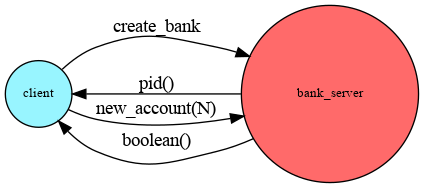
\includegraphics[width=0.75\textwidth]{create_bank-new_account.dot.png}
      \end{figure}
    \end{frame}

    \begin{frame}{Ejemplo práctico}
      \begin{figure}
        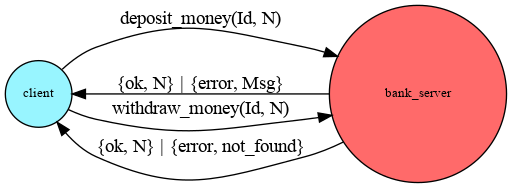
\includegraphics[width=0.75\textwidth]{deposit-withdraw_money.dot.png}
      \end{figure}
    \end{frame}

    \begin{frame}{Ejemplo práctico}
      \begin{figure}
        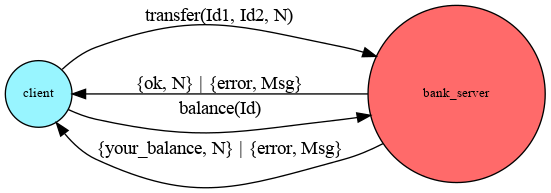
\includegraphics[width=0.75\textwidth]{transfer-balance.dot.png}
      \end{figure}
    \end{frame}

    \begin{frame}{Ejemplo práctico}
      \begin{figure}
        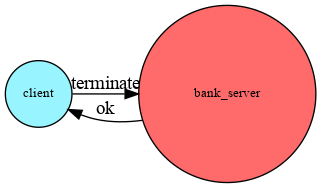
\includegraphics[width=0.75\textwidth]{terminate.dot.png}
      \end{figure}
    \end{frame}

    \begin{frame}[fragile]{Ejemplo práctico. Implementación}
      \begin{minted}[fontsize=\small]{erlang}
        %% API
        create_bank() -> spawn(fun() -> loop([]) end).

        terminate(Pid) ->
        Pid ! {terminate,self()},
        receive
          Msg -> Msg
        end.

        new_account(Pid,AccountNumber) ->
          Pid ! {new_account,AccountNumber,self()},
          receive
            Msg -> Msg
          end.
      \end{minted}
    \end{frame}

    \begin{frame}[fragile]{Ejemplo práctico. Implementación}
      \begin{minted}[fontsize=\small]{erlang}
        withdraw_money(Pid,AccountNumber,Quantity) ->
          Pid ! {withdraw_money,AccountNumber,Quantity,self()},
          receive
            Msg -> Msg
          end.

        deposit_money(Pid, AccountNumber,Quantity) ->
          Pid ! {deposit_money,AccountNumber,Quantity,self()},
          receive
            Msg -> Msg
          end.
      \end{minted}
    \end{frame}

    \begin{frame}[fragile]{Ejemplo práctico. Implementación}
      \begin{minted}[fontsize=\small]{erlang}
        transfer(Pid,FromAccount,ToAccount,Quantity) ->
          Pid ! {transfer,FromAccount,ToAccount,Quantity,self()},
          receive
            Msg -> Msg
          end.

        balance(Pid,Account) ->
          Pid ! {balance,Account,self()},
          receive
            Msg -> Msg
          end.
      \end{minted}
    \end{frame}

    \begin{frame}[fragile]{Ejemplo práctico. Implementación}
      \begin{minted}[fontsize=\small]{erlang}
        loop(Accounts) ->
          receive
            {new_account,AccountNumber,From} ->
              case proplists:lookup(AccountNumber,Accounts) of
                none -> %% Podemos crear esa cuenta
                  From ! true,
                  loop([{AccountNumber,0}|Accounts]);
                {AccountNumber,_} -> %% Ya existe esa cuenta
                  From ! false,
                  loop(Accounts)
                end;
            ...
      \end{minted}
    \end{frame}

    \begin{frame}[fragile]{Ejemplo práctico. Implementación}
      \begin{minted}[fontsize=\small]{erlang}
        {withdraw_money,AccountNumber,Quantity,From} ->
          case check_balance(AccountNumber,Accounts) of
            none -> %% No existe la cuenta
              From ! {error, not_found},
              loop(Accounts);
            Balance when Quantity =< Balance->
              From ! {ok,Quantity},
              UpdatedAccount = {AccountNumber,Balance-Quantity},
              NewAccounts = lists:keyreplace(AccountNumber,1,
                              Accounts, UpdatedAccount),                             ),
              loop(NewAccounts);
            Balance when Quantity > Balance ->
              From ! {error, not_money},
              loop(Accounts)
          end;
          ...
      \end{minted}
    \end{frame}

    \begin{frame}[fragile]{Ejemplo práctico. Implementación}
      \begin{minted}[fontsize=\small]{erlang}
        {deposit_money,AccountNumber,Quantity,From} ->
          case proplists:lookup(AccountNumber,Accounts) of
            none -> %% No existe la cuenta
              From ! {error, not_found},
              loop(Accounts);
            {AccountNumber,_} ->
              Balance = proplists:get_value(AccountNumber,Accounts),
              NewBalance = Balance + Quantity,
              From ! {ok,NewBalance},
              NewAccounts = lists:keyreplace(AccountNumber,1,
                              Accounts,{AccountNumber,NewBalance}),
              loop(NewAccounts)
          end;
          ...
      \end{minted}
    \end{frame}

    \begin{frame}[fragile]{Ejemplo práctico. Implementación}
      \begin{minted}[fontsize=\tiny]{erlang}
        {transfer,FromAccount,ToAccount,Quantity,From} ->
          case check_balance(ToAccount,Accounts) of
            none ->
              From ! {error, to_account_not_found},
              loop(Accounts);
            ToBalance ->
              case check_balance(FromAccount,Accounts) of
                none ->
                  From ! {error, from_account_not_found},
                  loop(Accounts);
                FromBalance when Quantity =< FromBalance ->
                  NewFromBalance = FromBalance - Quantity,
                  NewToBalance = ToBalance + Quantity,
                  From ! {ok,Quantity},
                  NewAccounts = lists:keyreplace(FromAccount,1,
                                  lists:keyreplace(ToAccount,1,
                                    Accounts,{ToAccount,NewToBalance}),
                                  {FromAccount,NewFromBalance}),
                  loop(NewAccounts);
                FromBalance when Quantity > FromBalance ->
                  From ! {error, from_account_not_money},
                  loop(Accounts)
              end
          end;
          ...
      \end{minted}
    \end{frame}

    \begin{frame}[fragile]{Ejemplo práctico. Implementación}
      \begin{minted}[fontsize=\small]{erlang}
        {balance,Account,From} ->
          case proplists:lookup(Account,Accounts) of
            none ->
              From ! {error,not_found},
              loop(Accounts);
            {Account,_} ->
              Balance = proplists:get_value(Account,Accounts),
              From ! {your_balance, Balance},
              loop(Accounts)
          end;
          ...
      \end{minted}
    \end{frame}

    \begin{frame}[fragile]{Ejemplo práctico. Implementación}
      \begin{minted}[fontsize=\small]{erlang}
          {terminate, From} ->
            From ! ok,
            ok;
          Unknown ->
            io:format("Unexpected message: ~p~n",[Unknown]),
            loop(Accounts)
          end.
      \end{minted}
    \end{frame}

    \begin{frame}[fragile]{Ejemplo práctico. Pruebas}
      \begin{minted}[fontsize=\small]{erlang}
        1> Bank = bank:create_bank().
        <0.86.0>
        2> bank:new_account(Bank, 1).
        true
        3> bank:new_account(Bank, 2).
        true
        4> bank:deposit_money(Bank, 2, 50).
        {ok,50}
        5> bank:withdraw_money(Bank, 1, 20).
        {error,not_money}
      \end{minted}
    \end{frame}

    \begin{frame}[fragile]{Ejemplo práctico. Pruebas}
      \begin{minted}[fontsize=\small]{erlang}
        6> bank:transfer(Bank, 2, 1, 30).
        {ok,30}
        7> bank:balance(Bank, 2).
        {your_balance,20}
        8> bank:balance(Bank, 1).
        {your_balance,30}
        9> bank:withdraw_money(Bank, 1, 20).
        {ok,20}
        10> bank:balance(Bank, 1).
        {your_balance,10}
        11> bank:terminate(Bank).
        ok
      \end{minted}
    \end{frame}

    \begin{frame}{Ejemplo práctico}
      \begin{itemize}
        \item Este ejemplo es la manera más ``explícita'' de implementar
        un servidor con estado
        \item Existen \textit{behaviors} dentro del lenguaje para construir
        este tipo de arquitecturas
      \end{itemize}
    \end{frame}

  \section{Conclusiones}
    \begin{frame}{Conclusiones}
      \begin{itemize}
        \item Erlang y MPI no resuelven los mismos problemas
        \item Erlang ofrece diversos mecanismos para crear aplicaciones
        concurrentes, con alta disponibilidad y fialibidad
      \end{itemize}
    \end{frame}

  \section{Bibliografía}
    \begin{frame}{Bibliografía}
      \begin{itemize}
        \item Getting Started with Erlang \url{https://www.erlang.org/doc/getting_started/intro.html}
        \item Learn You Some Erlang for Great Good! - Fred Hébert \url{https://learnyousomeerlang.com}
        \item Erlang Programming - Francesco Cesarini \& Simon Thompson
      \end{itemize}
    \end{frame}
\end{document}
